
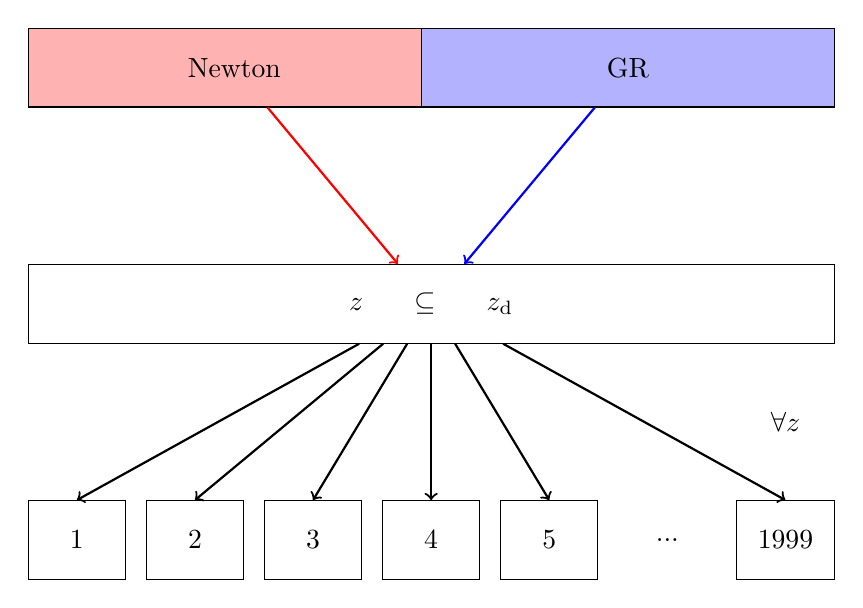
\begin{tikzpicture}
    \node[draw, rectangle, fill=red!30, text width=5cm, text centered, minimum height=1cm] (newton) at (0,3) {Newton};
    \node[draw, rectangle, fill=blue!30, text width=5cm, text centered, minimum height=1cm] (gr) at (5,3) {GR};

    \node[draw, rectangle, fill=white, text width=10cm, text centered, minimum height=1cm] (redshifts) at (2.5, 0) {$z\subseteq z_\mathrm{d}$};

    \draw[->, thick, red] (newton) -- (redshifts);
    \draw[->, thick, blue] (gr) -- (redshifts);


    \node[draw, rectangle, fill=white, text width=1cm, text centered, minimum height=1cm] (s1) at (-2,-3) {1};
    \node[draw, rectangle, fill=white, text width=1cm, text centered, minimum height=1cm] (s2) at (-0.5,-3) {2};
    \node[draw, rectangle, fill=white, text width=1cm, text centered, minimum height=1cm] (s3) at (1,-3) {3};
    \node[draw, rectangle, fill=white, text width=1cm, text centered, minimum height=1cm] (s4) at (2.5,-3) {4};
    \node[draw, rectangle, fill=white, text width=1cm, text centered, minimum height=1cm] (s5) at (4,-3) {5};
    \node at (5.5,-3) {...};
    \node[draw, rectangle, fill=white, text width=1cm, text centered, minimum height=1cm] (s1999) at (7,-3) {1999};

    \draw[->, thick] (redshifts) -- (s1.north);
    \draw[->, thick] (redshifts) -- (s2.north);
    \draw[->, thick] (redshifts) -- (s3.north);
    \draw[->, thick] (redshifts) -- (s4.north);
    \draw[->, thick] (redshifts) -- (s5.north);
    \draw[->, thick] (redshifts) -- (s1999.north);
    \node at (7, -1.5) {$\forall z$};

    
\end{tikzpicture}
